\section{Literature Review}
\subsection{Cognitive Load Theory (CLT)}
Cognitive Load Theory, primarily developed by John Sweller, suggests that since the human brain has limited \gls{working_memory} capacity, instructional design can aid in avoiding overload.
\textcite{sweller1988cognitive} proposes a three-part load framework that identifies three different types of cognitive load that impact a learner's ability to process information:

\begin{enumerate}
    \item Intrinsic Load~(\gls{IL}): This is the inherent difficulty of the task itself. It is defined by the number of elements must be processed 
    simultaneously to understand a concept. For example, learning basic vocabulary has low \gls{IL}, while mastering complex syntax has high \gls{IL}.
    \item Extraneous Load~(\gls{EL}): This is seen as the unnecessary load that you would aim to minimise wherever possible. It is influenced by the way 
    information is presented. Some examples that could exacerbate the load are poorly designed diagrams, distracting environments or redundant
     text. Poor design choices force the brain to waste resources on non-essential processing.
    \item Germane Load~(\gls{GL}): This is the load I am aiming to maximise. It refers to the mental effort that can be directed toward the more key task, 
    which in this scenario would be the code programming task.
\end{enumerate}

The framework can be simplified down to the idea that the Total Cognitive Load~(\gls{TCL}) is the sum of \gls{IL}, \gls{EL}, and \gls{GL}. 
The goal of instructional design is to manage these loads effectively to maximise learning outcomes.
$$TCL = IL + EL + GL$$

\begin{figure}[H]
    \centering
    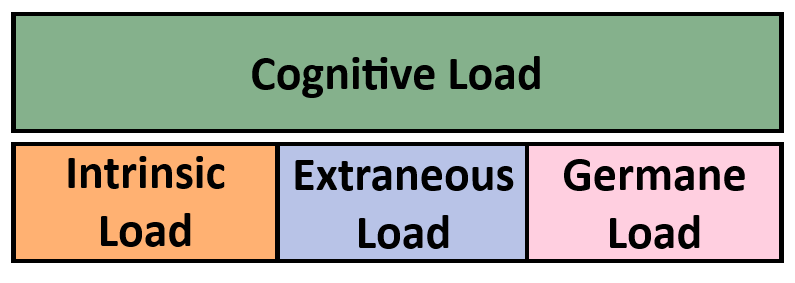
\includegraphics[width=0.8\linewidth, alt={A diagram illustrating Sweller's Tripartite Model. It shows Total Cognitive Load as a header, supported by three equal categories: \gls{IL} (task difficulty), \gls{EL} (presentation noise), and \gls{GL} (knowledge construction).}] {logos/clt_diagram.png}
    \caption{Sweller's Tripartite Model of Cognitive Load, illustrating the balance between Intrinsic, Extraneous, and Germane loads.}\label{fig:clt_diagram}
\end{figure}

While Sweller's Cognitive Load Theory provides the theoretical foundation, the application of these principles to \gls{neurodivergent} developers requires 
a more nuanced approach. One of the main focuses of this project is that for these developers, the \gls{IDE} environment often imposes a 
disproportionate \gls{EL}. When \gls{EL} is high, the cognitive budget is exhausted before the developer can engage with the core logic of the code, leading to \gls{task_paralysis}. 
My plugin aims to free up this mental bandwidth by suppressing \gls{EL} (via the Minimalist Toggle) and \gls{scaffolding} \gls{IL} (via the Task Architect),
thereby maximising the availability of cognitive resources for Germane processing. By reducing the noise and providing structured support, the plugin allows \gls{neurodivergent} developers to focus
their cognitive resources on the actual problem-solving aspect of programming, rather than being overwhelmed by the interface or the complexity of the task at hand.

\subsection{Applying CLT to \Gls{neurodiversity}}
For \gls{neurodivergent} developers, the \gls{EL} is not just due to bad design, but a barrier to entry. Features like the Activity Bar and Mini-map, while useful for some, can
be filtered out by a neurotypical developer but act as visual noise for those with \gls{ADHD} or \gls{ASD}.
To be able to code a high \gls{IL} is required. However, if the activation energy to start is too high due to \gls{executive_dysfunction}, the developer 
never reaches the stage where they can handle that load.
Having a single switch that closes all UI elements will directly targetC the suppression of \gls{EL} to free up mental bandwidth instantly without having to navigate menus.
While the \gls{AI} task decomposition tool acts as a cognitive prosthetic that scaffolds the \gls{IL} of project planning, preventing \gls{task_paralysis}.


\subsubsection{Integration with Rosenshine`s Principles of Instruction}

While Sweller provided the theoretical framework, Barack Rosenshine provided a \textit{how-to} to be used in classrooms or digital 
environments~\cite{rosenshine2012principles}. 

Main connections to Sweller`s principles include:

\begin{itemize}
    \item Small Steps (Principle 2): By presenting new material in small increments, the instructor limits the \gls{IL}, ensuring the 
    \gls{working_memory} is not overwhelmed at the outset.
    \item \Gls{scaffolding} (Principle 7): Providing temporary supports reduces \gls{EL}, allowing the learner to focus their cognitive 
    resources on the core task rather than the noise of the process.
\end{itemize}

To view these from more of a development lens, principle 2 supports breaking down the core task into smaller, more manageable steps. 
Further more these smaller task can be seen as \gls{scaffolding} for the user when they are beginning a task without handing them the answer directly.


\subsubsection{The Cognitive Theory of Multimedia Learning (CTML)}
While Sweller’s Cognitive Load Theory focuses primarily on the nature and management of cognitive load, Mayer`s \gls{CTML}~\cite{mayer2005cognitive} 
provides a more detailed explanation of how information is processed across visual and auditory channels. Within the context of software development, the
\gls{IDE} can be understood as a high-density multimedia environment in which multiple streams of related information must be processed simultaneously.

Within this framework, Ayres and Sweller`s split-attention principle describes the split-attention effect as occurring when learners are required to divide their attention 
between physically separated yet cognitively related sources of information~\cite{AyresSweller2021}. In a software development context, this may occur when an error message 
in the console refers to a line of code located hundreds of lines away in the editor. For a \gls{neurodivergent} developer, this creates a significant spatial split, requiring 
additional mental effort to navigate between and mentally integrate these sources of information. This integration process contributes directly to extraneous cognitive load, 
as cognitive resources are expended on locating and connecting information rather than resolving the underlying programming problem.

To mitigate this, the plugin`s \textit{Code Explainer} feature will provide an integrated view that combines the error message with the relevant code context, effectively 
reducing the split-attention effect. By presenting the error message and the associated code in a unified interface, the plugin minimises the need for mental integration
 across separate sources, thereby reducing extraneous cognitive load and allowing developers to focus more effectively on problem-solving.


\subsection{\Gls{neurodiversity} in Software Engineering}
To best design an inclusive plug-in, I needed to gain a deep understanding of the specific cognitive roadblocks faced by \gls{neurodivergent}
 developers. Recent research by \textcite{verma2025differences} and \textcite{gama2025socio} highlights that developers with \gls{ADHD}, 
 \gls{ASD}, and \gls{dyslexia} face significantly higher frequency of interruptions and difficulty obtaining knowledge.

\subsubsection{The Cognitive Load Connection}

For a \gls{neurodivergent} developer, a standard \gls{IDE} error message often carries a high \gls{EL}. What a neurotypical developer
 might perceive as a simple notification, a \gls{neurodivergent} individual may experience as a wall of cryptic text, inconsistent highlighting, 
 and ambiguous phrasing. This noise competes for limited \gls{working_memory} resources, leaving little room for the \gls{IL} required actually 
 to solve the logical problem.

\subsubsection{Executive Functioning and Task Switching}

\Gls{executive_dysfunction} is a primary barrier cited by both~\textcite{verma2025differences} and~\textcite{gama2025socio}. This manifests
 itself as difficulty in \gls{task_initiation} (starting a new project) and switching between tasks.

\textbf{The Industry Context:} In a modern software environment, developers are rarely afforded the luxury of a single focus; they must
 balance code reviews, meetings, and multiple projects.

\textbf{The Impact:} For those with \gls{ADHD}, the mental cost of having to remember the context of a project after an interruption is significantly higher. If the \gls{IDE} does not provide clear "waypoints" or historical context, the developer may become cognitively paralysed, unable to determine where they left off.

\subsubsection{Specific Challenges by Condition}

Based on the synthesis of recent studies, the challenges can be categorised as follows:

\textbf{\gls{ADHD}}: Frequent loss of state due to external interruptions and internal distraction.\textcite{verma2025differences} found that these developers report higher stress related to waiting for answers, as delays in information retrieval often lead to a total loss of task momentum.

\textbf{\gls{ASD}}: Challenges with the \Gls{double_empathy} problem in code, where the high-level abstractions or implied logic used by neurotypical colleagues create a high cognitive overhead for autistic developers who prefer explicit, literal documentation.

\textbf{\Gls{dyslexia}}: Significant hurdles during the syntax-heavy stages of programming. While these developers often excel at high-level architectural mapping, the \gls{EL} of spelling-sensitive compiler errors and dense documentation can be a major deterrent to productivity.

\subsubsection{Beyond Medical}

To understand why existing tools fail, we  must examine the shift from the \Gls{medical_model} to the \Gls{social_model}.

\begin{itemize}
    \item \textbf{The \Gls{medical_model}}: Traditionally, \gls{ADHD} or \gls{dyslexia} in engineering has been viewed as a deficit to be corrected through individual coaching or medication.
    \item \textbf{The \Gls{social_model}}: This perspective argues that the developer is disabled not by their neurology, but by an \gls{IDE} designed with a \gls{neurotypical-bias}. The problem is not the individual's
     brain, but the environment that fails to accommodate it. This shift in perspective is crucial for designing tools that are not just assistive but truly inclusive, as it focuses on modifying the
      environment (the \gls{IDE}) rather than trying to fix the individual.
\end{itemize}

The minimalist toggle and the code explainer are designed with this \gls{social_model} in mind, aiming to create an environment that reduces barriers and allows \gls{neurodivergent} developers to thrive 
without needing to conform to a neurotypical standard.

\Gls{EF} Domains in Programming
To deepen the analysis of \gls{executive_dysfunction}, we must break it into three core domains:
\begin{itemize}
    \item \textbf{Inhibitory Control}: The ability to ignore distractions. For \gls{ADHD} developers, the \textit{pop-up} notifications of a linter can break a fragile state of focus.
    \item \textbf{\Gls{working_memory}}: Dyslexic developers often have a high capacity for 3D spatial reasoning but a limited verbal \gls{working_memory}, making syntax-heavy languages like C++ more taxing than cleaner languages like Python.
    \item \textbf{Cognitive Flexibility}: The ability to switch between thinking about the big picture architecture and the low-level syntax.
\end{itemize}

\subsubsection{The Double-Edged Sword of \Gls{hyperfocus}}
While \gls{neurodivergent} developers, particularly those with \gls{ASD} and \gls{ADHD}, are often stereotyped as having a \textit{superpower} for deep work, 
this ability to \gls{hyperfocus} is more accurately described as a dysregulation of attention. Unlike the psychological concept of \textit{flow} which is
 generally sustainable and self-directed, \gls{hyperfocus} is an involuntary immersion into a task or activity. As noted by~\textcite{gama2025socio}, \gls{hyperfocus} allows 
for an exhaustive exploration of complex problems, yet this intensity often comes at the expense of self-care. Developers may neglect fundamental 
biological needs, such as nutrition, sleep, and hygiene, leading to rapid burnout. 

In the context of software engineering, this creates a High-Intensity/High-Fragility paradox.~\textcite{newman2025get} identifies that for \gls{ADHD} programmers, achieving a flow state is a fragile process where a single interruption can collapse hours of built-up mental context. The subsequent \gls{state_recovery_cost} is significantly higher 
for \gls{neurodivergent} individuals, often leading to burnout or irritability when the state is broken.

In a professional engineering context, this creates a significant conflict between depth and delivery. \Gls{hyperfocus} can inadvertently trigger over-engineering, 
where a developer becomes locked into optimising a single component while neglecting broader project milestones or team collaborations. This inability to switch 
off from an interesting problem makes task-switching, a fundamental requirement of agile development, mentally exhausting and practically difficult. Consequently, 
what appears to be peak productivity from the outside is often an unsustainable trade-off that risks both the developer's well-being and the project's timeline.

\subsection{Existing Tools}
The design of \glspl{IDE} often follows a one-size-fits-all model, which inherently leads to a \gls{neurotypical-bias}, creating barriers for those who may 
require additional support.~\textcite{morris2015understanding} observes workplace tools are frequently built with assumptions that ``may not align with 
the needs of \gls{neurodiverse} employees.'' \glspl{IDE} are often packed with tools that enable customisation; however, they are not designed with \gls{neurodiverse} 
developers in mind, and complex nested menus can be overwhelming.

Despite the obstacles described, certain features provide essential support for developers.~\textcite{morris2015understanding} notes that tools such as code 
completion and linters are vital to alleviate the difficulties associated with \gls{dyslexia}, such as syntax memorisation and spelling.

However, the burden of making tools accessible often falls to the user.~\textcite{liebel2024challenges} found that developers often create ``individual
 strategies and tool configurations to support their productivity''. While these features are currently helping, the reliance on manual customisation 
 implies a lack of \textit{out-of-the-box} inclusivity.

This project aims to bridge the gap between the availability of generic tools and their functional utility. While current tools are excellent at
 detecting errors, they often fail at explaining them in an accessible manner. By integrating an Error Explainer that decomposes complex compiler 
 messages into manageable tasks, therefore reducing the cognitive load required to debug. This shifts the \gls{IDE} from a passive environment that 
 requires expert configuration to an active partner in the development process.

\subsection{Pomodoro Timer}
The Pomodoro Technique, developed by Francesco Cirillo~\cite{cirillo2018pomodoro} in the late 1980s, is a time-management framework that partitions work into focused intervals. Typically
25 minutes, separated by brief five-minute breaks. In the context of \gls{neurodiversity}, this method is often reframed as a cognitive tool rather than a rigid 
rule set, specifically designed to address common \gls{EF} barriers~\cite{miller2025wired}.

\subsubsection{Managing \Gls{executive_dysfunction} and \Gls{task_paralysis}}
For developers with \gls{ADHD} or \gls{ASD}, \gls{task_paralysis}, an inability to initiate work due to cognitive overload or anxiety represents a significant hurdle. 
The Pomodoro Technique mitigates this by lowering the activation energy required to start. By committing to a manageable, 25-minute sprint, the psychological 
barrier to entry is reduced, helping individuals bypass the freeze response associated with daunting or abstract tasks.

\subsubsection{Combatting \Gls{time-blindness} and \Gls{hyperfocus} Burnout}
\Gls{neurodivergent} individuals often experience \gls{time-blindness}, a difficulty in perceiving the passage of time as a concrete resource. Externalising time through a visual 
or auditory timer provides real-time feedback, helping to anchor the developer to the present task and reducing the risk of underestimating project timelines.

Furthermore, while \gls{hyperfocus} can lead to severe mental and physical exhaustion if left unregulated. The structured 
nature of the Pomodoro cycle acts as a release valve for focus:
\begin{itemize}
\item Mandatory Breaks: Frequent breaks prevent the \gls{hyperfocus} trap, where a developer may neglect basic biological needs like nutrition or hydration.

\item Sensory Regulation: Scheduled pauses provide essential space for sensory recovery, allowing developers to move around to prevent the physical strain and irritability that often follow hours of sedentary deep work.
\end{itemize}

\subsubsection{Cognitive Load and Adaptive Implementation}
From the perspective of Cognitive Load Theory (CLT), the Pomodoro Technique manages mental resources by preventing the exhaustion of the cognitive budget. By breaking a 
complex project into small, time-limited stages, the method reduces \gls{EL}, the unnecessary effort required to manage a vast, unstructured task, allowing for more 
\gls{GL} to be directed toward core algorithmic problem-solving.

However, In some cases it could be argued that the standard Pomodoro settings can sometimes be counterproductive if applied too rigidly. For individuals with \gls{ADHD}, 
a 25-minute window may be too short to enter a productive flow state, leading to \glspl{state_recovery_cost} if interrupted too early. To address this, the plugin
 will allow users to customise the length of their focus intervals and breaks, providing flexibility to accommodate different working styles and cognitive needs.

\subsection{Colour filters}
Visual presentation can influence reading performance and comfort.~\textcite{griffiths2016effect} found that coloured overlays may reduce visual stress for some readers, 
although the benefits vary significantly between individuals. This suggests that software tools should support flexible visual customisation rather than relying on a single accessibility configuration.

In some cases, high-contrast models are essential because they provide the necessary visual \gls{scaffolding} to combat \gls{task_paralysis}. For developers with \gls{ADHD}, a low-contrast or pastel theme can
cause code elements to bleed together, increasing the cognitive effort required to distinguish between keywords, variables, and logic.
By utilising high-contrast ratios such as 7:1 or higher, per \gls{WCAG} 2.1 guidelines the \gls{IDE} creates a clear visual hierarchy.

This high signal environment provides several technical advantages:
\begin{itemize}
    \item Reduce Visual Search Time: Finding the start and end of a function block becomes instantaneous rather than a manual scan.
    \item Mitigate the Blur of \Gls{hyperfocus}: As noted by~\cite{newman2025get}, the intense mental strain of being in the groove can lead to visual fatigue; high contrast maintains legibility even as physiological focus wanes.
    \item Support Syntax Logic: In complex, nested code, high-contrast separation between brackets and operators serves as a visual prosthetic, offloading the work of pattern recognition from the brain to the interface.
\end{itemize}

\subsubsection{The \Gls{halation} Risk and Soft High Contrast}
While high contrast is vital for clarity, pure high contrast (e.g., stark white text on a pure black background) can be counterproductive for those with \gls{ASD} or specific visual stresses.
 This combination can cause \gls{halation}, a glowing or bleeding effect around letters that makes text appear to vibrate or move~\cite{cruz2025empiricalinvestigationexperiencesdyslexic}.

 To address this, the most effective models for \gls{neurodiversity} are often \textit{Soft High Contrast} themes. These utilise high-visibility colors against deep, non-pure-black backgrounds 
 (such as dark greys or navy). This balance provides the necessary signal for \gls{ADHD} developers to maintain focus while preventing the sensory overwhelm and visual distortion common in \gls{ASD} profiles.
However, the implementation must be nuanced in order to avoid \gls{halation}.
Therefore, the most effective high-contrast models for \gls{neurodiversity} are often \textit{Soft High Contrast}, utilising high-visibility colours against deep non-pure-black backgrounds.

\subsection{\gls{AI} as a Cognitive Tool: Task Decomposition and \Gls{scaffolding}}
For developers with \gls{ADHD} and \gls{ASD}, the most significant barrier to productivity is often not the complexity of the code itself, but the executive function tax required to organise a project. 
Research by \textcite{newman2025get} indicates that \gls{ADHD} professional programmers specifically struggle with state recovery and \gls{task_initiation}.~\glspl{LLM} offer a unique solution to this 
through cognitive \gls{scaffolding}. This process handles the \textit{low-value} mental energy drains, such as formatting and scheduling, leaving more room for \textit{high-value} deep thinking (\cite{Navigati93:online}).

Instead of asking a model to simply write a function, the developer can use the model to decompose a broad, abstract goal into a granular, step-by-step plan. This process mitigates the \textit{activation energy} barrier identified in \gls{ADHD} populations. By prompting a model to 
think step-by-step, the \gls{AI} generates a logical roadmap for the developer to work through, as well as referring back to it if the task is interrupted.

As noted by \textcite{Navigati93:online}, this automated pattern of \gls{scaffolding} can increase productivity for developers with \gls{ADHD}. Existing tools already demonstrate this by taking a single
 overwhelming command (e.g., ``build an authentication system'') and breaking it into manageable milestones. This effectively transforms \gls{AI} from a simple code generator into a digital ramp that bypasses 
 the freeze response common in \gls{task_paralysis}.

 \subsection{NASA-TLX and SUS: Measuring Cognitive Load and Usability}
To evaluate the effectiveness of the plugin, I will use the NASA Task Load Index (\gls{NASATLX}) to measure cognitive load and the \gls{SUS} to assess usability.
The \gls{NASATLX} provides a multidimensional assessment of perceived workload across six dimensions: Mental Demand, Physical Demand, Temporal Demand, Performance, Effort, and Frustration.
This will allow me to quantify the reduction in cognitive load achieved by the plugin. The \gls{SUS}, on the other hand, is a widely used tool for assessing the usability of systems and interfaces.
It consists of a 10-item questionnaire that provides a global view of subjective assessments of usability. By using both tools, I can gain insights into how well the plugin reduces cognitive
 load while also ensuring that it is user-friendly and accessible for \gls{neurodivergent} developers.

 I have chosen these tools because they are well-established in the field of human-computer interaction and provide a comprehensive framework for evaluating both the cognitive and usability
  aspects of the plugin. The \gls{NASATLX} will help me understand the specific areas where cognitive load is reduced, while the \gls{SUS} will provide feedback on the overall user experience. 
  This dual approach ensures that the plugin is not only effective in reducing cognitive load but also meets the usability needs of its target audience.

\subsection{Curb-Cut Principle and Universal Design}
When it comes to accessibility it is often cited that all users, including those without specific disabilities, can benefit from accessible design principles.
\textcite{johnson2003creating} illustrate the concept using the classic example of the curb-cut principle. This term was coined from ramps and dips in curbs originally 
designed for people using wheelchairs. However, it is also used by people pushing strollers, pulling luggage, and rollerbladers making the accessibility benefits fit a broader audience.
The same principle applies to software design.~\textcite{reid2024curb} notes that the curb-cut effect is associated with the Universal Design movement, which advocates for technology to be 
designed to be accessible and usable by disabled and non-disabled people alike~\cite{null2013universal}.

In the context of this project, the plugin's features, such as the Minimalist Toggle and Code Explainer, are designed to reduce cognitive load for \gls{neurodivergent} developers. 
However, these features also have the potential to benefit neurotypical developers by providing a cleaner interface and clearer error explanations. By applying the curb-cut principle, 
the plugin aims to create an inclusive environment that enhances the user experience for all developers, regardless of their accessibility needs.
